\documentclass[spanish]{article}
\usepackage[spanish]{babel}
\usepackage{amsmath}
\usepackage{amssymb}
\usepackage[utf8]{inputenc}
\usepackage{vmargin}
\usepackage{graphicx}
\usepackage{wrapfig}
\usepackage[export]{adjustbox}


\begin{document}

\includegraphics[width=1\textwidth, right]{./imagenes/logos.png}
	\setpapersize{USletter}
	\setmarginsrb{30mm}{30mm}{30mm}{30mm}{0pt}{0mm}{0pt}{0mm}
	
	\begin{center}
	{\Large Análisis de Algoritmos, Sem: 2018-1, 3CV2 Práctica 6, 19 de Octubre del 2017}\\
{\huge {\bf Práctica 6: Problema del Maximo Subarreglo}} \\
{\large {\bf Salgado Alarcon Genaro, Padilla Calderon Jose Manuel}\\
Escuela Superior de Cómputo \\
Instituto Politécnico Nacional}\\
isomaelking@gmail.com, genaro\_yen13@hotmail.com\\
	\end{center}

	
	\bigskip
	
	\bigskip
	
	\bigskip
	
	{\LARGE {\bf Primero}}\\
	
	En este trabajo vamos a demostrar la complejidad del algoritmo de maximo subarreglo, al igual que uno de sus parientes el de maximo subarreglo cruzado, estos seran tratados tanto de manera grafica como de manera analitica, los resultados que estamos esperando son los de un algoritmo de maximo subarreglo cruzado con complejidad lineal, en el caso del algortimo de maximo subarreglo una complejidad de $\theta(nlogn)$, ademas de considerar el caso cuando el arreglo esta lleno con numeros enteros negativos, en el cual sabemos se presenta un caso interesante.

	\bigskip


	{\Large {\bf Palabras Clave}}\\
	\begin{itemize}
		\item Algoritmo
		\item Funcion
		\item Recursividad
		\item Orden
		\item Arreglo
	\end{itemize}
	
	\section{Introducci\'on}
	El término Divide y Vencerás en su acepción más amplia es algo más que una
	técnica de diseño de algoritmos. De hecho, suele ser considerada una filosofía
	general para resolver problemas y de aquí que su nombre no sólo forme parte del
	vocabulario informático, sino que también se utiliza en muchos otros ámbitos.
	El enfoque de Divide y venceras que evidentemente es mejor cuanto mas grande es el caso, lo cierto es que puede resultar mas lento que el algoritmo clasico en casos que sean 			demasiado pequenos. por tanto el algoritmo de divide y venceras debe de evitar seguir avanzando recursivamente cuando el tamaño de los casos no lo justifique.

\newpage
	\section{Conceptos B\'asicos}
	Para la correcta comprension de este trabajo, es necesario definir algunos terminos tales como $\theta$, O y $\Omega$.\\
	 $\theta$(n):\\
		Sea g(n) una función. Se define  $\theta$ (g(n)) como:\\
		
		 	$\theta$(g(n)) = $\{ f(n) \quad | \quad \exists c1,c2>0 \quad \& \quad n_{0}>0 \quad \mid \quad \forall n>=n_{0} \quad 0<= c1g(n) <= f(n) <= c2g(n) \}$
	\bigskip		 	
		 	
	O(n):\\
		Sea  g(n)  una función, O(n) (el pero de los casos) se define como:\\
		
			\hspace{1cm}O(n)=$\{f(n) \quad | \quad \exists c >0 \quad \& \quad n_{0}>0 \quad | \quad f(n) <= Cg(n) \quad \forall  n>= n_{0} \}$
	\bigskip
	
	$\Omega$(n):\\
	Sea  g(n)  una función. Se define $\Omega$ (g(n)) (el mejor de los casos) como:\\

		\hspace{1cm}$\Omega$(g(n)) =$\{f(n) \quad | \quad \exists c >0 \quad \& \quad n_{0}>0 \quad \mid \quad  0<= cg(n)<= f(n) \quad \forall n>= n_{0} \}$
	\bigskip

	El problema del maximo subarreglo nos dice que dados varios numeros que supondremos estan almacenados en un arreglo, se trata de encontrar la secuencia de numeros contiguos cuya suma sea maxima.\\
	Ahora pondremos un ejemplo muy sencillo con el arreglo A que podemos apreciar en la Fig1.\\
	\begin{center}
		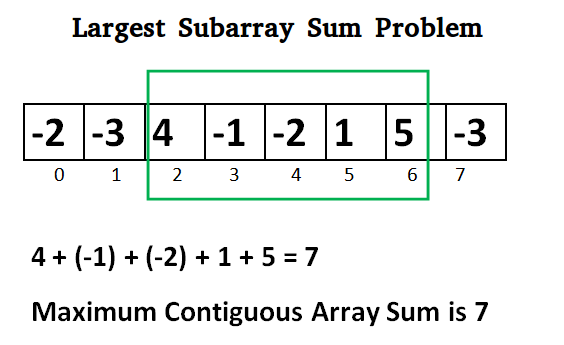
\includegraphics[width=0.55\textwidth]{./imagenes/fig1.png}\\
		Figura 1. Arreglo A .\\
	\end{center}
	El maximo subarreglo de este arreglo A seria, la seccion que vemos en la Fig 2, cuya suma es igual a 25.\\
	\begin{center}
		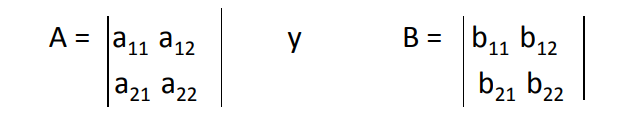
\includegraphics[width=0.25\textwidth]{./imagenes/fig2.png}\\
		Figura 2. Maximo subarreglo del arreglo A .\\
	\end{center}
	Ahora si existe mas de una solucion, nos conformaremos con hallar una de ellas.
	\newpage	

	\section{Experimentaci\'on y Resultados}
	
	\subsection{Implemente el algortimo del maximo subarreglo.}
	
	{\large{ {\bf i) Mediante gráficas, muestre que el algoritmo de  ${\bf maximo subarreglo cruzado}$ tiene complejidad lineal.}}}\\

	\bigskip

	*****

	\bigskip

	{\large{\bf ii)  Demuestre analíticamente que el algoritmo  ${\bf maximo subarreglo cruzado}$ tiene complejidad lineal.}}\\
	
	\bigskip
	
	*****

	\bigskip

	{\large{\bf iii) Mediante gráficas, muestre que el algoritmo  ${\bf maximo subarreglo }$ tiene complejidad ${\bf \theta(nlogn)}$.}}\\
	
	\bigskip
	
	*****

	\bigskip

	{\large{\bf iV) Demuestre  analíticamente que el algoritmo  ${\bf maximo subarreglo }$tiene complejidad ${\bf \theta(nlogn)}$.}}
	
	\bigskip
	
	*****

	\bigskip

	{\large{\bf V) Implemente un algoritmo que resuelva el problema del máximo subarreglo utilizando fuerza bruta. Calculé su orden de complejidad analítica y experimentalmente.}}\\
	
	\bigskip
	
	*****

	\bigskip

	\newpage

	\bigskip

	\section{Conclusi\'on General}

	\bigskip

	*****

	\bigskip

	\section{Conclusiones Individuales}

	\bigskip

	{\large{\bf Salgado Alarcon Genaro}}\\

	\bigskip

	*****

	\bigskip

	{\large{\bf Padilla Calderon Jose Manuel}}\\
	
	\bigskip

	******	

	\bigskip

	\newpage

	\section{Anexos:}
	

	{\large 1.  ¿Qué retorna la función del máximo subarreglo cuando todos los valores son enteror negativos?}\\

	\bigskip

	\section{Bibliografía}
	\begin{itemize}
		\item Brassard, G. (1997). Fundamentos de Algoritmia. España: Ed. Prentice Hall. ISBN 		848966000X
		\item Harel, D. (2004). Algorithmics: The spirit of Computing (3rd. Ed). Estados Unidos de América: Addison
Wesley. ISBN-13: 978-0321117847
	\end{itemize}


\end{document}